\chapter{Discussion and Future Work}
\label{Discussion}

\section{Introduction}
\label{Discussion:Intro}

\begin{figure}[htp]
\centering
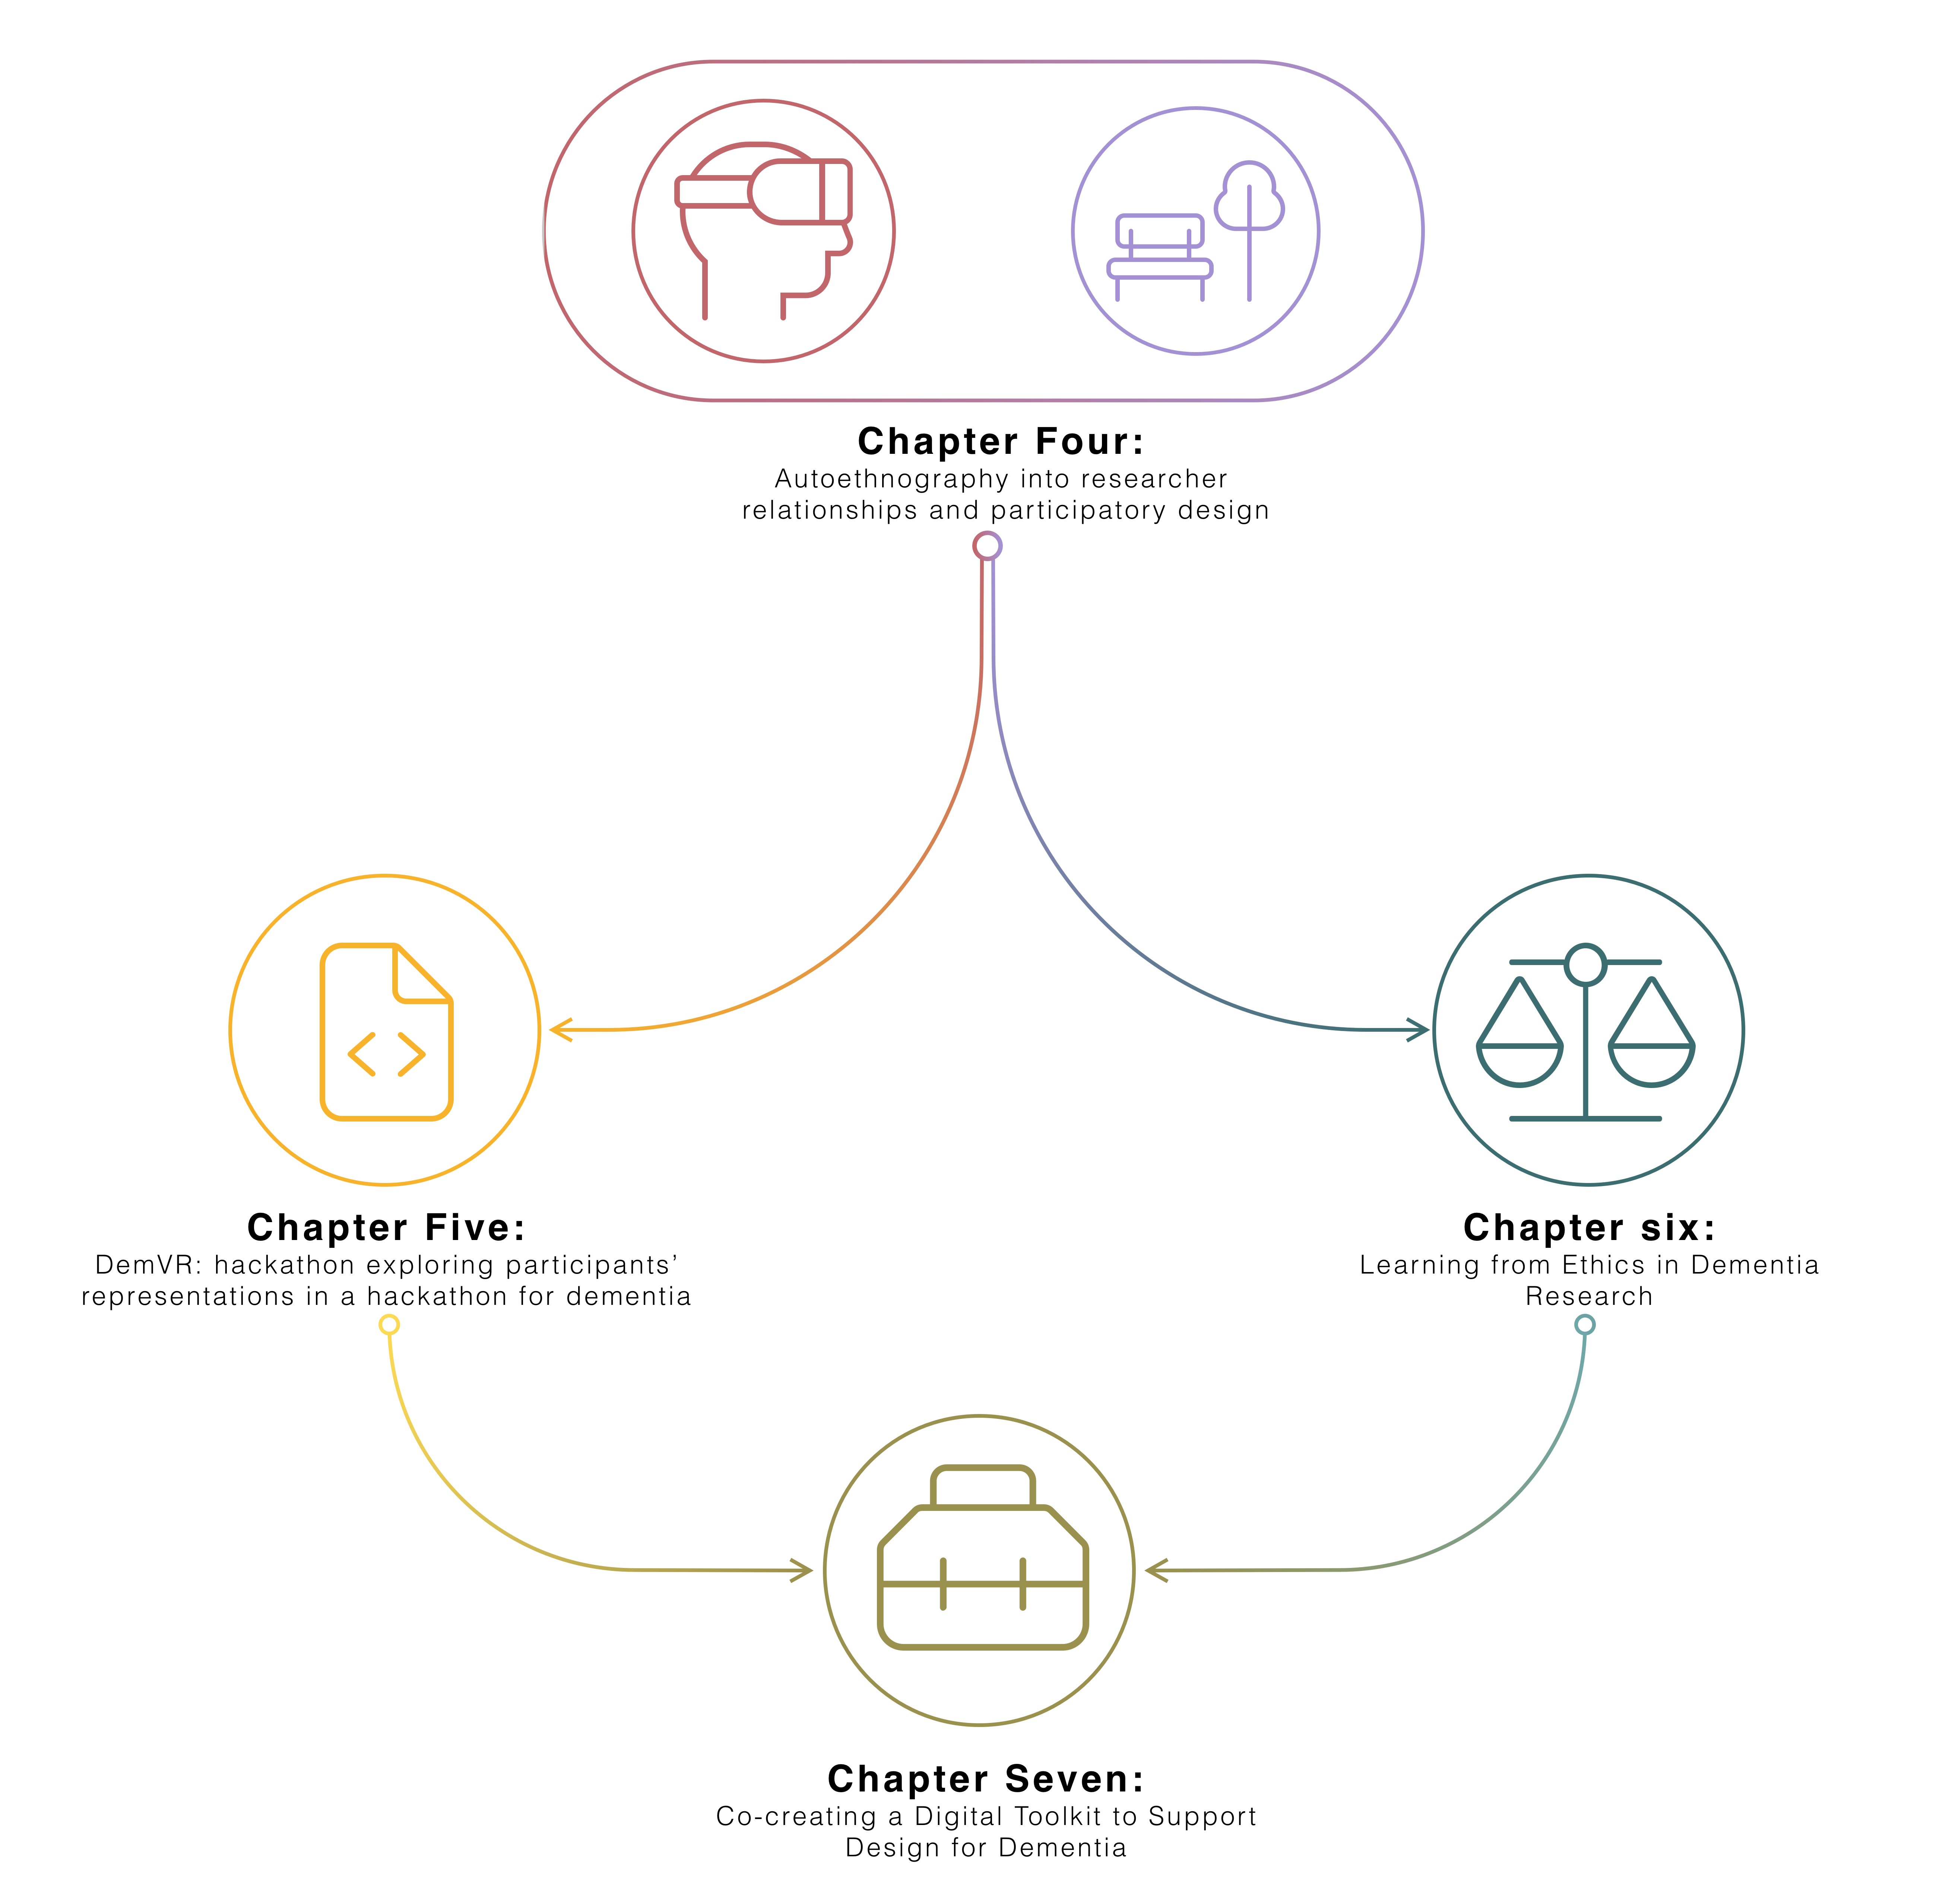
\includegraphics[width=0.8\linewidth]{Images/Thesis_Narrative/Narrative_Full.png}
\caption{data chapter flow}
\label{fig:NarrativeFlow}
\end{figure}

In this thesis, I have broadened the conversation around dementia and HCI to capture the views of care partners, designers, developers, researchers, the public, and people with dementia. The importance of providing a shared set of experiences and understandings stems from the prior work that emphasises how we might \textit{"enrich and deepen the story about the situation of people with dementia"} \citep{bartlett2010broadening} by considering a more relational perspective through individuals who make choices and influence everyday interactions with people with dementia. Within the literature, I describe the evolving role of co-design and participation in dementia and HCI research that was once oriented to the individuality of the person with dementia, has recently begun to point towards widening our view of dementia towards a more sociological-oriented perspective that requires exploration into societal structures and relationships that affect the person with dementia \citep{lazar_critical_2017}. 

Following the literature, I describe the four data chapters that aim to tackle the research questions set out in the introduction. In case study one, I examine the different relationships between myself, dementia charity and the families with dementia that I recruited. Within this chapter, I co-design a series of VR and media experiences that emphasise the importance of attending to the person with dementia's interests and desires and that of the family and friends. Through this work, I explore the day-to-day interactions and understand how technology can provide more nuanced and shared experiences that provide a more enabling role of shared decision-making. From exploring working with families with dementia, I raised a set of questions and awareness on the ethical complexities in conducting dementia research and the long-term relationship building required to co-create meaningful media technologies that encompassed individuals' interests. In response, the subsequent two chapters tackle particular issues found in chapter four (seen in fig.\ref{fig:NarrativeFlow})

For chapter five, I explore public engagement with the topic of dementia, I ran a two-day hackathon called DemVR, which aimed to provide a space for participants to design novel use cases of shared Virtual Reality (VR) experiences for people with dementia and their care partners. Much of dementia research emphasises the importance of relationships and sensitive design to support close and personal interactions. However, this approach requires long term engagement between researchers and participants that is often a small representative of individuals who are part of those communities that the researcher reached out to. In this chapter, I revisit the hackathon structure to reflect on how the work practices led to a lack of involvement of people with dementia and their care partners. In the analysis of interview and ethnographic data, I provide insight into the motivations for those taking part in hackathons, and an account of how some participants new to the area of dementia conceptualised, operationalised, and designed for an absent user. 

For chapter six, I invited 22 researchers from the dementia and HCI practice to come together to elucidate wider concerns about ethics in HCI research. In contrast, I describe several concerns in chapter four, chapter six gains an understanding from diverse countries, institutions and disciplines. The findings uncover tensions arising from institutional ethical practices in socially oriented research. While ERBs vary significantly in their cultural and disciplinary approaches to dementia research, the findings reveal the tensions that arise in participatory research due to ERBs’ tending to focus on the protection of participants, which raises concerns with acknowledging participants and building relationships. Through our interviews, researchers reflected on how ERBs could be more reflexive bodies, where researchers can seek support, guidance, and
collaboration from experts. Researchers also shared insights from their own cultivated practices from establishing clear expectations for participants, knowing when and how to involve participants in the research, and appropriately acknowledging the contribution that participants make to our work. From these rich findings, the chapter progresses from a growing body of work in HCI and dementia towards establishing a new set of fluid ethical practices to direct work in this growing area of socially-oriented HCI research.

In the final data chapter, a key concern that was central to my prior work was how dialogue is curated between public, designers, developers and people with dementia to ensure that the development of dementia technology has involved people with dementia in meaningful ways. Working with seven designers, four developers, and five people with dementia, I invited participants to participate in a three-stage iterative process to explore the type of resources developers and designers need to design with people with dementia and investigate how people with dementia envision their potential participation within a toolkit. Following stages one and two, we used a process of affinity diagramming to help surface a set of design priorities to guide our design for a final dementia design toolkit prototype – which I called the Dialogical Dementia Design (D3) Toolkit. Within this toolkit, I provide several activities to provide designers/developers with an ethical and sensitive way to engage with people with dementia dialogically, opportunities to reflect and critically think about relevant aspects of dementia and provide curation of toolkit resources to be community-driven through the inclusion of varying stakeholders' involvement. Following the toolkit design, I conducted a final workshop inviting participants to reflect on the prototype toolkit to provide further insights into how designers, developers and people with dementia may contribute, use, and envisage how toolkit components might facilitate co-creation between different groups. 

In the remainder of this thesis, I revisit the main research question:
\begin{quote}
\textbf{\textit{"How might participation be configured for people with dementia to shape the design process of technology”}}
\end{quote}
The subsection below explores the lessons learned across the data chapters and are organised into the three individual research questions that tackled the overarching research question above. Following the review of each research question, I describe four 'future work' studies that build upon the individual data chapters to provide opportunities for future research.
\section{Participatory approaches}
\label{Discussion:RQ1}
\begin{quote}
\textbf{    Research Question 1:
}    
\textit{    “How can we use participatory design approaches to provide meaningful and engaging experiences for people with dementia?”}
\end{quote}

Throughout the thesis, I addressed participatory design approaches in various ways. Chapter four examined a series of participatory design approaches to engage with people with dementia and their families. Through working closely with the families, I adapted traditional participatory methods to fit the needs of the participants, such as creating family days out in which participants would take part in walking interviews. Following on from this work, I was motivated to explore how to broaden these participatory methods to function within the context of larger-scale community events seen in chapter five - that prompted me to explore how hackathons could provide a creative and inclusive space for the public to engage the topic of dementia. 

However, while I gained reasonable interest from designers, developers and students, the event significantly under-represented people with dementia and their care partners. The failure to represent and involve people with dementia in public engagement had multiple knock-on effects on teams' outputs. Still, it provided an opportunity to reflect on the appropriateness of hackathon structures for people with dementia and propose alternatives for collaborative design events. Finally, in chapter seven, I worked with people with dementia, designers, and developers to understand how these different stakeholders may collaborate in building technology. With this in mind, two considerations that arise in responding to the research question are: a) designing for authentic participation through creative means, and b) meeting your participants where they are.

\subsection{Designing for authentic participation through creative means}
\label{RQ1:Creativity}
As I have argued through this thesis, dementia and HCI has rapidly grown over recent years bringing design approaches to work with people with dementia to support language, cognitive and memory challenges. This has resulted in adapting well-established methods or developing new approaches tailored to the particular needs of the researcher's participants. For instance, in chapter four, I describe the co-design of days out with families who then took part in a set of walking interviews. Given the importance of verbal communication in traditional interviews, which can be quite stressful and memory oriented, these walking interviews provided opportunities to describe what they saw, felt, smelled, and heard during the walk \citep{kullberg2017walking}. Additionally, the families were exposed to conversational triggers regarding the environment that resonated with past and present memories.

Within dementia work that has creativity approaches as a central role in communication, use of creativity is often used to create a 'conversational space' to be shared by people with dementia and others. For instance, \cite{ferguson2014dementia} explored those with dementia who are further marginalised through being Deaf British Sign Language (BSL) users. By integrating themselves into the community and becoming active co-communicators to actively understand the voices, the researchers provided a safe and meaningful space for the deaf dementia community to open up about their cultural and linguistic minority to understand their lives better. Furthermore, the authors highlight that deaf people see non-verbal interactions as their way of being in the world and that we can learn a lot of creative approaches to fundamentally support people with dementia who are non-verbal.

As several researchers described in the findings of chapter six, many dementia and HCI researchers would redesign their methods to lean on creative and visual means as a way to interact in activities and researcher. In \cite{welsh_ticket_2018} work with intergenerational communication in dementia, the author argues that these technologies and methodologies provide the person with dementia an opportunity to be included in conversations where they are often ignored. While we have come a long way to engaging with people with dementia in many different ways, the later stages of the thesis made it apparent that the infrastructures and technology that many of us required through COVID-19 made engaging people with dementia challenging. Relying on embodied queues in communication over Zoom is often tricky, particularly to facilitate from afar without the tactile, touching and doing attributes attained from in-person interaction. Therefore, although we might be returning to in-person interactions, researchers should consider how technology may support non-verbal interactions and provide conversational assistance for meaningful and engaging interactions for people with dementia and their friends and family when using video-calling systems.

\subsection{Meeting your participants where they are}
\label{Discussion:WhereTheyAre}
In chapter four, I highlighted several concerns at the end of the study where the participants had lost that initial interest in developing VR technology despite expressing enjoyment in the participation and creation of the moment boxes. Additionally, in chapter five, I detail the deployment of Ideaboard, an online platform that I thought people with dementia and carers would use. In both instances, these assumptions to use VR, and an online platform came from my decisions rather than driven by agendas of the population. Instead of making assumptions on ways to engage with people with dementia, I suggest asking participants what platforms they would like to use for engagement. Not only does this reduce development costs, but this also provides the opportunity to understand the communication processes your participants are familiar with. 

One approach I might have adopted during the hackathon would be an ‘Unplatformed’ approach to designing the pre-hackathon experience and recruitment stage. Unplatformed design is a model for the appropriation of social media technologies, that pays particular attention to the implications of the individual features of social media in respect to coordinating participation in specific contexts \citep{lambton-howard_unplatformed_2020}. I might have reduced barriers to engagement and ensured better representation of the views of our participants by coordinating participation on the technologies that they were already comfortable with (e.g., Twitter, Facebook, and other media platforms). Although I knew that some community members whom we would have liked to have reached used these platforms, I were seeking an additional ‘string to our bow’ by piloting the use of the Ideaboard platform. Nevertheless, in this case, it hindered rather than increased participation. 

However, it should also be noted that utilizing solely digital methods to facilitate recruitment and engagement could be limiting for some participants facing significant marginalisation. For instance, \citep{lazar_safe_2019} describe how even inclusive initiatives centred around the involvement of people with dementia may silence voices that offer less "polished stories" or those who are nonverbal. \cite{dai2020making} describe that while online interactions provide an enjoyable and beneficial interaction for the person with dementia, it contributes to a burden and the need for the care partner to provide \textit{“responsive, continuous, and knowledgeable support|” (pg.46:24) \citep{hwang2020exploring}}. 

Moreover, we should consider ways to invite and involve participants in the research processes and recruitment stages to help ensure agendas and processes to engagement are more closely aligned with the participants. To this extent, participant-led research may offer understandings into new, more impactful ways our research be of benefit to communities beyond academic publications. Alongside, researchers should continue to provide additional context for their recruitment methods when working in sensitive settings to generate a set of knowledge on the challenges and possibilities of participant engagement in this area of work.

\section{Ethical implications in Dementia and HCI}
\label{Discussion:RQ2}
\begin{quote}
\textbf{    Research Question 2:
}    
\textit{    “What are the ethical implications for people with dementia to participate in HCI research?”}
\end{quote}
Across all the studies in this thesis, there has been ongoing ethical implications in how we involve and perceive people with dementia in HCI research. In particular, chapters four and six delve into such challenges in several ways. For chapter four,  I describe initial insights into my understandings of representation within dementia that encompasses my time at Silverline Memories and reflections on family history of dementia. As I explained at the end of chapter four discussion, the critical area that I felt underexamined was the ethical implications apparent in our work as a community of practice. This led to chapter six, where I invited 22 HCI and dementia researchers to reflect on their everyday experiences of working with people with dementia and the complexities that may arise in technology or institutional ethics. Through this thesis, exploring these ethical challenges led to more profound insights into the ways we represent and acknowledge people with dementia, and exploration into the 'ruling relations' that shape people with dementia's experiences. 

\subsection{Designing for contested realities}
\label{RQ2:ContestedRealities}
In chapters four and six, it was clear that working with people with dementia may present moments of individuals slipping in and out of realities which can then be contested by those around them, who struggle with these conflicting accounts of reality. In chapter four, I describe how Michael sometimes struggles to orient Lauren to reality, creating new experiences of grief when she is told, time and again, that her mother is dead. In contrast, Dana Walrath's graphic novel Aliceheimer's, about her relationship with her mother - Alice, who has Alzheimer's, conveys accepting her mother's reality and often going along with Alice's reality:

\begin{quote}
\textit{"[the graphics novel], shows how we treated Alice's hallucinations and disorientation as a special power. Instead of fighting about what was really there or where each of us was, we let her ability to travel through space and time peaceably account for our distinct realities. This made it possible for me to read the symbols buried in her travels. As I created the art, I used symbols such as cut text form Lewis Carroll's Alice in Wonderland to make Alice's bathrobe, her favorite garment, to convey our magical approach to living with dementia" \citep{walrath2021aliceheimer,walrath2017end}}
\end{quote}
Orienting the person with dementia towards the "right" reality has very little effect; if the dementia is sufficiently progressed, the person will simply forget this reorientation again. It is also considered to be poor practice \citep{cipriani_understanding_2014}. It is imperative to remember that a sense of self can come from more than just our ability to recall and recount memories. Working with people with dementia sensitively should push us to reflect on the structural challenges of understanding the reality of the person living with dementia and designing for this often' dreamlike' state, depending on the stage of dementia \citep{bryden_before_2015}. With this in mind, we should consider what it means to design media experiences for realities that may eclipse each other briefly rather than conflict with each other entirely. In a similar vein,  although in chapter four, I indicated how outside activities can be captured via media, I must stress that this is no substitute for going outside, or for care homes to replace (for instance) gardening or nature walks with virtual realities of the same. Actually engaging in such activities has multiple psychological and physiological benefits \citep{gilliard_transforming_2011} — we should instead begin to think about how both activities can overlap and eclipse each other: for instance, participants could collect rocks from beach walks — these are easily fitted with RFID tags which, when touched or otherwise triggered, lead to a change or simple interaction in the immersive environment.

\subsection{Designing 'to be with', not 'be like'}
\label{sec:considerationbeWith}
When working with designers and developers, a significant portion of the work has been trying to understand ways to provide individuals with insight into dementia. For instance, in chapter four, I spent a large portion of time at Silverline Memories, getting to know the individual members and understanding their lives with dementia to build my perspective of dementia and how HCI may benefit their lives. When it came to running the hackathon, I intended to bridge the gap between the gap and people with dementia by supporting conversations between them to scale the similar experiences I had in a shorter period. Due to the lack of involvement of people with dementia, teams' leaned on alternative approaches such as personas. 

While personas are beneficial in imagining the people you may be designing for, they are prone to stereotypes that is further emphasised to elucidate technological solutions to the challenges at hand. Further \cite{turner2011stereotyping} describes that \textit{"once a stereotype has been activated it can shape the predication's we make about people and situations".} As described in the findings, even the teams' with significant dementia research knowledge were prone to stereotypes for example while this is a well defined persona by team \textit{Sensory Tide}, it lends itself to appeal to 'priming' certain problem areas that the team want to tackle in their VR shared experience.
\begin{quote}
\textit{Mary is 81 and lives in Forest Hall with her husband Joe. She has two sons who live close by and visit her almost daily; her granddaughter Rachel also visits regularly with her 7-year-old daughter. Mary has been living with Alzheimer’s Disease for around 5 years now. She enjoys being social and being included in conversations, but it is sometimes clear that she doesn’t always follow what is being said. She will often forget people’s names and where she had put things, and can often get confused or lost if left alone. For the last few years her husband has been doing most of the household chores and caring for Mary, but he has recently had some health problems which means he is a lot less mobile. Both Mary and Joe enjoy being around people and being outdoors, but they now need to rely on other people to bring them places following Joe’s illness. Neither of them are particularly technology literate. Joe has a basic mobile phone for emergencies, but they do not own a computer. }
\end{quote}

While their persona paints a well defined person with dementia and it is apparent they are pulling from their vast knowledge of the area, making their personas \textit{"neither technology literate"} or the husband to be \textit{"doing most of the household chores and caring for Mary"} creates clear problem statements for the experience to fix such as their VR experience being assisted by the person with dementia's care partner, or an attempt to make VR technology as easy as possible to engage with. While they are important prompts to consider, it overlooks the possibilities of more enriching design responses such as teaching people with dementia and their care partners about technology to provide Independence towards not relying on others. 

In response, the final study explored how we might design toolkits and resources that offer opportunities for creativity and sympathy towards the users we are designing for rather than designing methods that attempt the developer or designer to feel or understand what it is like to live with dementia. Designing activities for meaningful dialogue between communities echoes the similarities to the IDEO deck of cards called 'Adapt-o-pack'. In this card game, users select from six different persona cards of a person with a disability and pair these with workplace settings such as farming that are intended to challenge the narrative of what people with disabilities can and can't do. The lead designer, Megan Durlak, states:

\begin{quote}
\textit{
It is impossible for a person without a disability to ever truly understand what it means to be disabled. Period. True empathy, however, can often take the form of human connection over a shared emotion or experience. The Adapt-o-Pack creates this moment of connection by tapping into the creative potential of the participant, and encouraging them to, even for a moment, empathize with the type of creative necessity people with disabilities display on a daily basis.
} \citep{durlak}
\end{quote}

Throughout the thesis, I have explored the different ways we may represent the voices of people with dementia and have argued (and learnt from the mistakes), that approaches that model or attempt to replicate what it feels like to have dementia are prone to stereotypes and inaccuracies in the representation of dementia. Instead, affective understanding between various stakeholders comes from potential partnership building to help designers and developers reimagine what 'dementia' represents and the potential contributions people with dementia and care partners can provide in the design process. 

\section{Supporting meaningful dialogue}
\label{Discussion:RQ3}
\begin{quote}
\textbf{    Research Question 3:
}    
\textit{ “What are the competing interests and expectations to support meaningful dialogue in dementia design research when involving multiple stakeholders - such as people with dementia, developers, designers and researchers?”}
\end{quote}
In my literature review on the representation of dementia in the public eye, it is common for people with dementia to be stigmatised surrounding their abilities to communicate and socialise with others. As discussed in chapter four, I adapted the interview approaches to suit the family's needs by co-design days out, which supported meaningful dialogue between myself and the families with dementia. However, on a more comprehensive approach to this research question, chapter five - DemVR, and chapter seven - designing a collaborative toolkit, directly considers ways to facilitate an engaging and meaningful dialogue between the public, designers, developers, and people with dementia. In both chapters, I facilitated conversations surrounding ways technology can promote dialogue between the public and people with dementia. Chapter five deployed an online platform - Ideaboard, where designers, developers, people with dementia and care partners could take part in short consultations to share ideas for VR experiences to be explored in the hackathon. As I report in the chapter, this was a disfavoured platform that was lacked the engagement I had hoped for. In the discussion, I highlight issues of participant disinterest and how the platform was not intentionally built with people with dementia in mind. 

For the final data chapter, I build upon these mistakes to consider what toolkits and technologies could we use to support dialogue between people with dementia and technologists. In conducting this work with designers, developers and people with dementia from the ground-up, the findings demonstrated two priorities for making meaningful dialogue between the different communities - appropriate incentives for all and designing for the ecology of care.

\subsection{Appropriate incentives for all}
\label{RQ4:Incentives}
During the prior studies, they have been several dicussions on the type of incentives that the different stakeholders may require to ensure meaningful involvement. For instance, in chapter four, the families' interest in the study came from being listened to and enjoyable day-out at their desired locations. Similarly, in the ethics study in chapter six, researcher's expressed different ways to recognise and compensate people with dementia's time that went beyond the typical money or voucher that is usually tied into research compensation. These forms of incentives stretched from providing meaningful experiences during the study, to acknowledging participants as authors of the academic paper. Regardless of how we recognise and design our incentives for people with dementia, we should recognise participants as individuals who have contributed their knowledge, experience and time.  

In contrast, the competition money provided a clear incentive for designers and developers within the hackathon. Within the findings, teams expressed a gradual change in their motivation once they had more experience with dementia \citep{gama2017crowdsourced}. For instance, VRHallucinate were motivated by the stark contrast of Howard's experiences where the team thought a diagnosis of dementia would bring support from \textit{"friends and [relationships] would be a lot closer…instead, there is a lot of loneliness surrounding it"}. Similarly, \citep{foley_student_2020} work on student engagement with residents at a care home, describes students "sense of purpose and the determination" where their role became a more supportive through the building of relationships by getting to know the residents.  

As teams sympathised and had their perceptions opened to the challenges and possibilities of living with dementia, Garden Life's motivations were driven by a desire to continue to \textit{"deepen [an] understanding of these issues" in hope to "help to alleviate the stigma"} that contributes to the misrepresentations of dementia. While prize money was a contributor to participating in the weekend, multiple teams indicated pro-social motivations while providing a unique collaborative space for learning and exploring the potential use cases of VR and dementia. In such a way, further consideration into longer-term relationships and learning may provide reciprocal incentives. 

However, while the hackathon provided incentive for designers and developers, it lacked insight into the type of incentives for people with dementia and care partners. For chapter seven when building the lo-fi toolkit, it was clear that involving people with dementia recognised that people with dementia want to support the knowledge and creation of that content that designers and developers may use in their design processes. Reflecting on the lack of output the hackathon provided, preparing the event with the community may have offered us additional insights into understanding the topics of interest and the type of technologies that may be of use. Further, working with the community may have provided other alternatives for a hackathon. While I intended to understand hackathons in the dementia context, the funding provided this opportunity could have been used to support engagement between schools and care homes or contribute to funding to maintain dementia communities that are perhaps doing more for dementia than a public hackathon. 

\subsection{Designing for the ecology of care}
\label{R4:EcologyOfCare}
In the early stages of this thesis, I emphasised how we might design for the different needs of the person with dementia, their families, friends, and caregivers. For chapter four, I designed the media experience not only for and with people with dementia but also for their family members. This is in contrast to other studies in HCI and dementia, which tend to focus on the person with dementia as the recipient of the designed object or technology. When carers are designed for/with, the technologies are typically more focused on care duties. Similarly, little attention was given to care partners' values, expectations, and needs during the hackathon. While this may have been a knock-on effect of the event having a central focus on 'designing VR experiences for dementia', it undermines the importance that care partners have in adopting technology and overlooks the individuality of the care partner.

In one study, Michael (care partner), told me a story of his past, which focuses on his own experiences, not those experiences by his partner Lauren:
\begin{quote}
\textit{"We ended up in a little village called Farnworth. And in Farnworth there's a stream that runs through it. There is a road bridge, and underneath the road bridge, there is a deep place where you can get your horse in and you can wash all its legs off and get all of the mud off the bottom of it. Then . . . [a lady] went right under, which of course was hilarious to some of us who were still slightly uninhibited. But I can see the whole thing in my mind. It was just a fun day. It's all down to 150\% whiskey spirit."}
\end{quote}
While creating the moment boxes for the families, I preserved Michael's memory by including it in an edited audio segment to value the ecology of care around the person with dementia and the person themselves. In dementia, our close and familial relationships can be constitutive of ourselves \citep{wallace_making_2013}, and many carers report high levels of burnout and burden \citep{takai_experience_2009}. Targeting carers as research participants worthy of digital interventions means treating them with respect and whole persons rather than defining them by their roles. With this in mind, in chapter seven, while I stress the importance of building tools to promote conversation between designers, developers and people with dementia, we should also be acknowledging the role of family, friends and care partners who will likely support the person with dementia's interactions. 

\section{Future work}
\label{FutureWork}
The following section builds on the four data chapters to move beyond the abstract discussions found in the previous data chapters to present four evocative studies for future work within technology and dementia. Through these prospective studies, I have attempted to articulate what the abstract directions I have suggested may entail acting as inspiration for researchers who wish to build onto this work. In each future study, I propose a research question with a clear explanation of how this ties into prior work found in this thesis and why it is important for the future of dementia and HCI. The four ideas are not an exhaustive list, nor an attempt to design studies that will answer all the questions generated through this thesis. Rather, they are starting points for researchers who may explore areas of VR, community design events, learning of ethics, and public representation of dementia through storytelling.

\subsection{Ageing in a virtual world}
\label{FutureStudyOne}
\begin{figure}[htp]
\centering
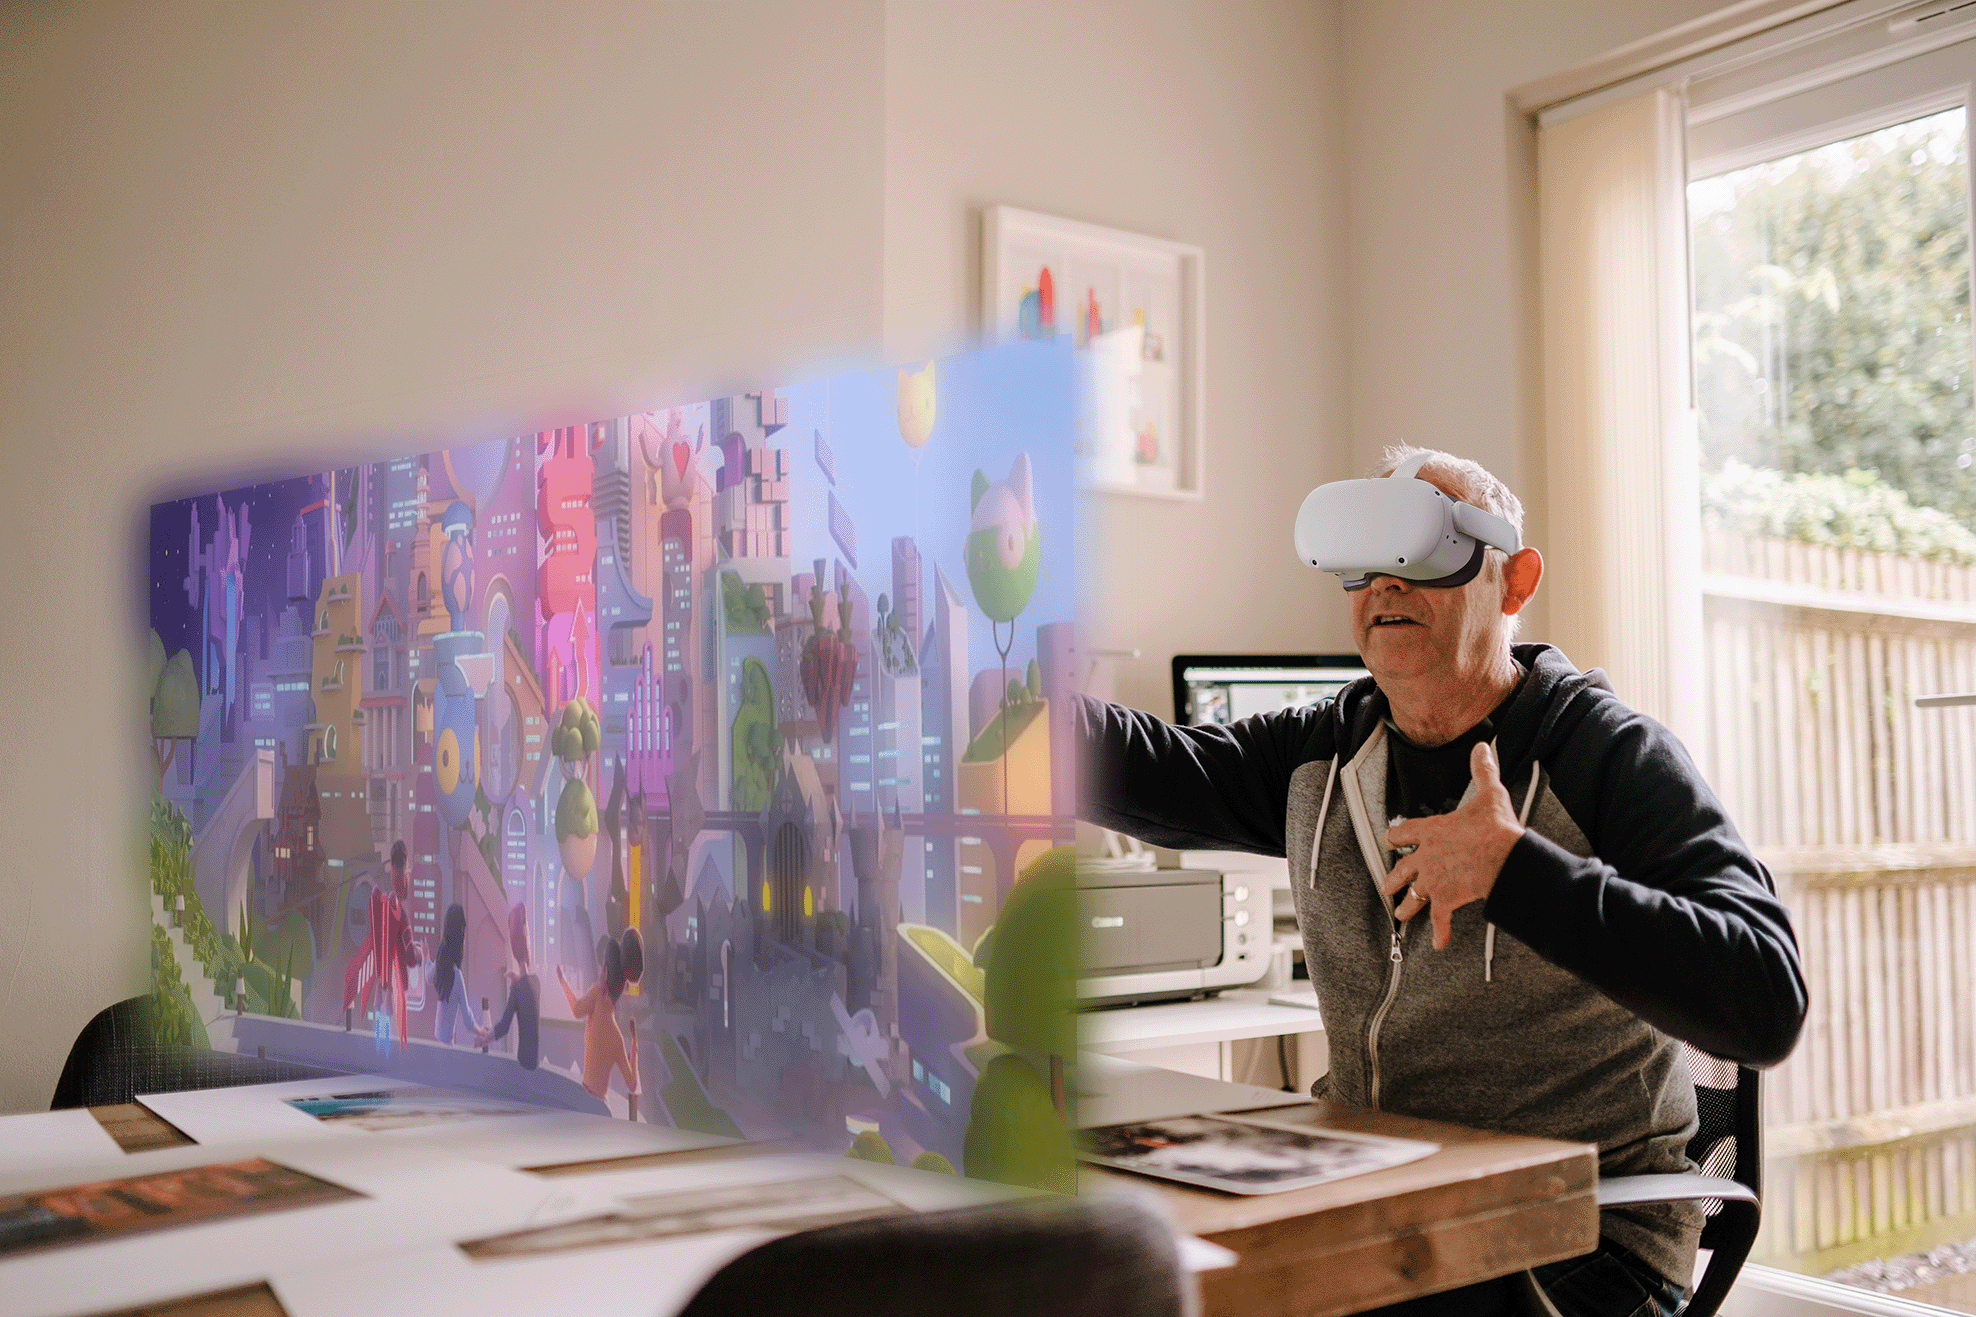
\includegraphics[width=1\linewidth]{Images/Discussion/Aging_in_VR.png}
\caption{Older adult exploring VR spaces}
\label{fig:Aging_VR}
\end{figure}
As mentioned in chapter four, the findings provided insight into several participants feeling a lack of confidence when getting out and about, due to the progression of their dementia. As we age, our body typically degrades as well, and people with dementia are often "reduced" to the bodily as their communicative abilities change and they move into care. Kontos describes much of the life of nursing homes in terms of their embodied potential. For instance, choosing to dress in specific ways, participating in the sleep-wake cycle of nursing homes, the attempts of care workers to transform (via various methods) residents into 'docile, dementing bodies' \citep{kontos_embodiment_2013,kontos_relational_2017}. However, \cite{twigg2009clothing} describe clothing provides a strong sense of selfhood and communication through embodied interactions:

\begin{quote}
\textit{"Age has always been a one of the key structuring principles, and we should not be surprised to find it reflected at the bodily level in the clothes that people wear. Indeed, part of the wider role of clothes, as we noted, is to render social difference concrete and visible. But these traditional forms of age ordering are increasingly under pressure. The democratisation of fashion and the growth of involvement of older people in consumption are in the process of changing the nature of age ordering in dress in ways that point to wider shifts in the experience and understanding of later years." }\citep{twigg2009clothing}
\end{quote}

Twigg positions the body as a site for knowing the world - which can be fruitful when we consider designing VR experiences for people with dementia. With this in mind, a research question that has yet to be explored is \textbf{\textit{"How might we emphasise active ageing and representation of people with dementia through their designing of virtual avatars"}}. In chapter six - DemVR, multiple teams felt conflicted in fantasy elements and providing virtual hands and heads within the VR environment for different users. Ultimately, as described in the findings, the teams prioritised the safety of the person with dementia as they assumed people with dementia might feel uneasy with floating avatars that represent the user. However, in a recent study by \cite{mendez2015virtual}, people with dementia communicated through their virtual avatars, including answering questions and conversing in the conversation between multiple virtual participants.

As VR continues to work with the popularity and investment into the 'metaverse' \citep{kraus2022facebook}, for some, using VR avatars is becoming an everyday interaction through virtual meeting rooms, playing online games with friends, to socialising in virtual spaces with strangers and friends. While there have been recent steps in improving virtual interactions between avatars, such as the new 'personal boundary' features to VR avatars to prevent others from creeping into the user's personal space \citep{sharma_2022}, there is a lack of work into how we may age with these avatars. Do we preserve physical ailments and disabilities that often accompany dementia? Do we provide avatars that age over time in the same way our physical bodies do? Progressing in this area will mean careful co-design intervention that pays attention to the bodily as a means to communicate just as well as the verbal.

\subsection{Design with Inclusion}
\label{FutureStudyTwo}
\begin{figure}[htp]
\centering
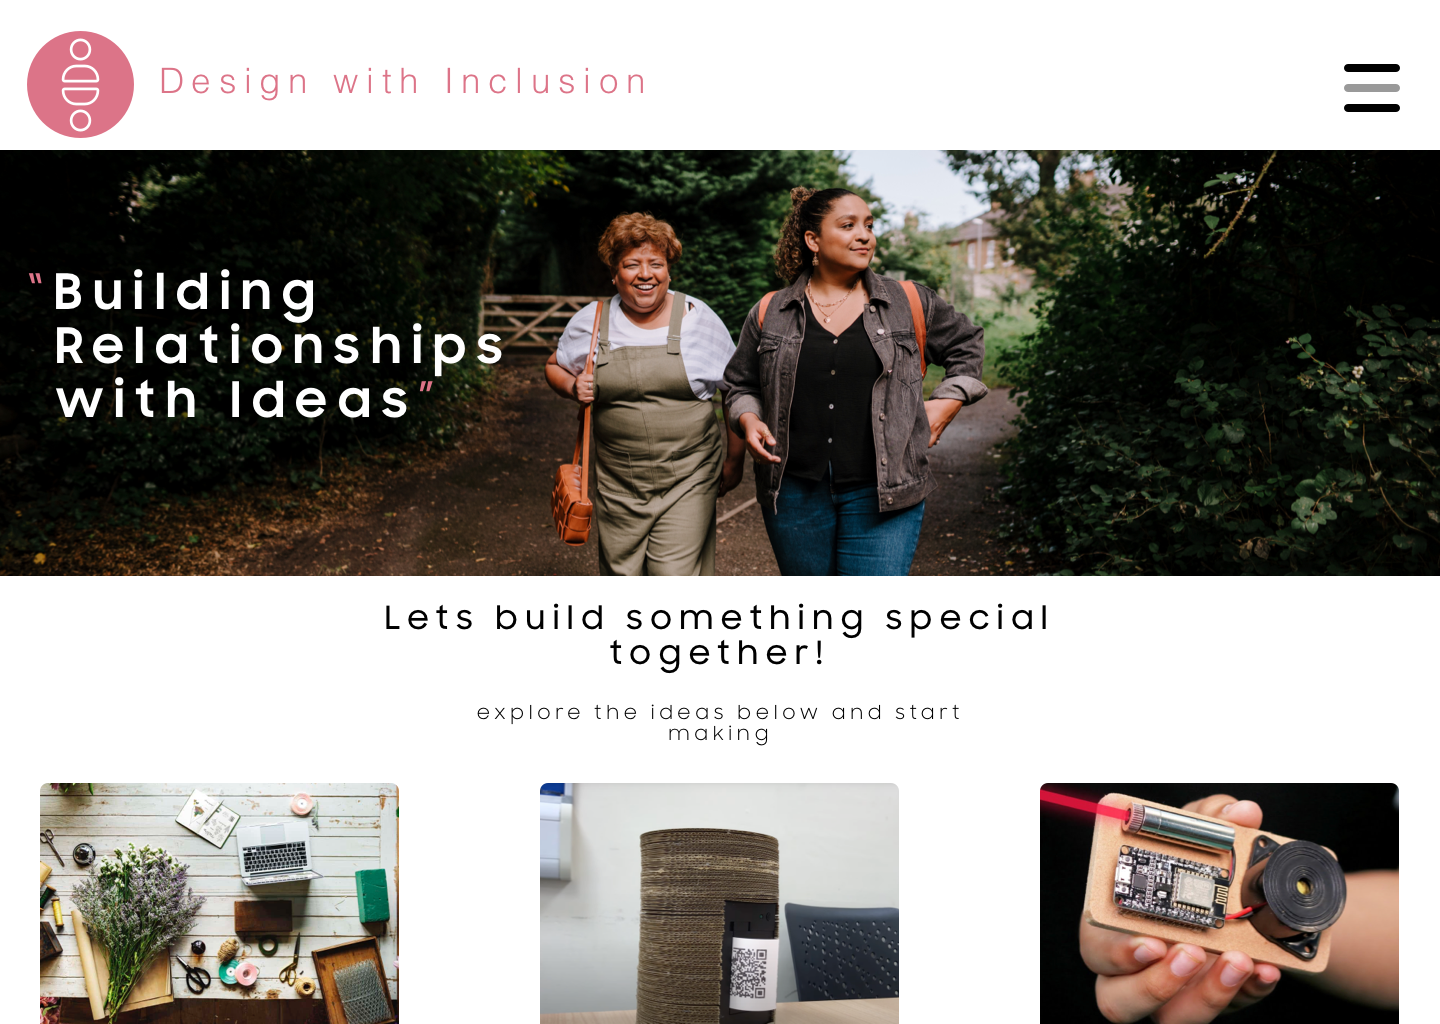
\includegraphics[width=1\linewidth]{Images/Discussion/Design_For_Inclusion.png}
\caption{Design with Inclusion website mockup}
\label{fig:DesignInclusion}
\end{figure}
One way forward in collaborative digital design for communities undergoing significant challenges might be to promote the growth of loosely coupled, companion 'communities of practice'. In chapter five - DEMVR, the makeup of many teams, which seemed to be themselves drawn from discrete, already existing communities; for example, undergraduates from the same computer science course; researchers from multimedia labs; and filmmakers. For design research for older age or in dementia, the idea of partnering communities together – for instance, partnering a cohort of design or technology students together with a community of older people, and having both mutually learn from one another – may hold promise. The UK-based 'FixEd' \citep{noauthor_fixperts_nodate}, for instance, has introduced a scalable learning programme called 'Fixperts' that targets schools and universities to engage their students in creative problem-solving that is rooted in the communities around them – for example, a student might engage with an older neighbour to innovate simple solutions that fit into their current lives, which help them get out of a car; or another student might work with someone experiencing a time-limited disability or injury to help them safely navigate their college campus. Capitalising on the ingenuity and availability of design, technology and engineering students looking for meaningful application areas, such programmes deliver small-scale, bespoke fixes for potentially large numbers of people. Similar ideas are seen at work in programmes such as TimeBanking \citep{noauthor_hour_nodate}, and even within studies previously cited such as \cite{reuter_older_2019}, which made use of the resources a university is often rich in (e.g., technical competence, A/V equipment) to innovate within a radio programme for older people, leading them to encourage researchers 'to consider participatory action research as a method of assistance in itself, complimented by technical innovation to facilitate processes in this space'.

Given the interest in dementia as an area of interest for design and technology students, a study that might consider \textit{\textbf{"How might we facilitate and promote different communities to 'partner-up' to share knowledge and skills?"}} In figure \ref{fig:DesignInclusion}, I have mocked up a website called 'Design with Inclusion' that builds up the challenges found in chapter five. It has been argued that older adults and people with dementia tend to adopt more DIY or ‘off the shelf’ products instead of using health and social care services. Although this largely stems from services not considering client’s needs, DIY solutions provide cheaper and tailored products that fulfil a particular problem \citep{gibson2015everyday}. Reflecting on the hackathon, an alternative approach would have been to let people with dementia and families to post ideas for DIY solutions that could have been built over a short period where designers and developers could share their skills in building the solution. Providing space for the different communities may have provided a more reciprocal relationship where designers learnt about dementia and lived experiences. In contrast, care partners and people with dementia would end up with a DIY project that they could use at home. Furthermore, by tailoring the interactions to be focused on personalised smaller scale products that tackle a particular challenge the user is facing, this may move away from fear for participants sacrificing their big hackathon idea to a university/organisation. By developing programmes of participation that are extended in time, organised around a common purpose, and provide meaningful benefits for student-practitioners, real, even incremental, change for a community of people with dementia. This may well be a more inclusive, ethical way to approach innovation and impact within this space.

\subsection{Suggestive guidance pack}
\label{FutureStudyThree}
\begin{figure}[htp]
\centering
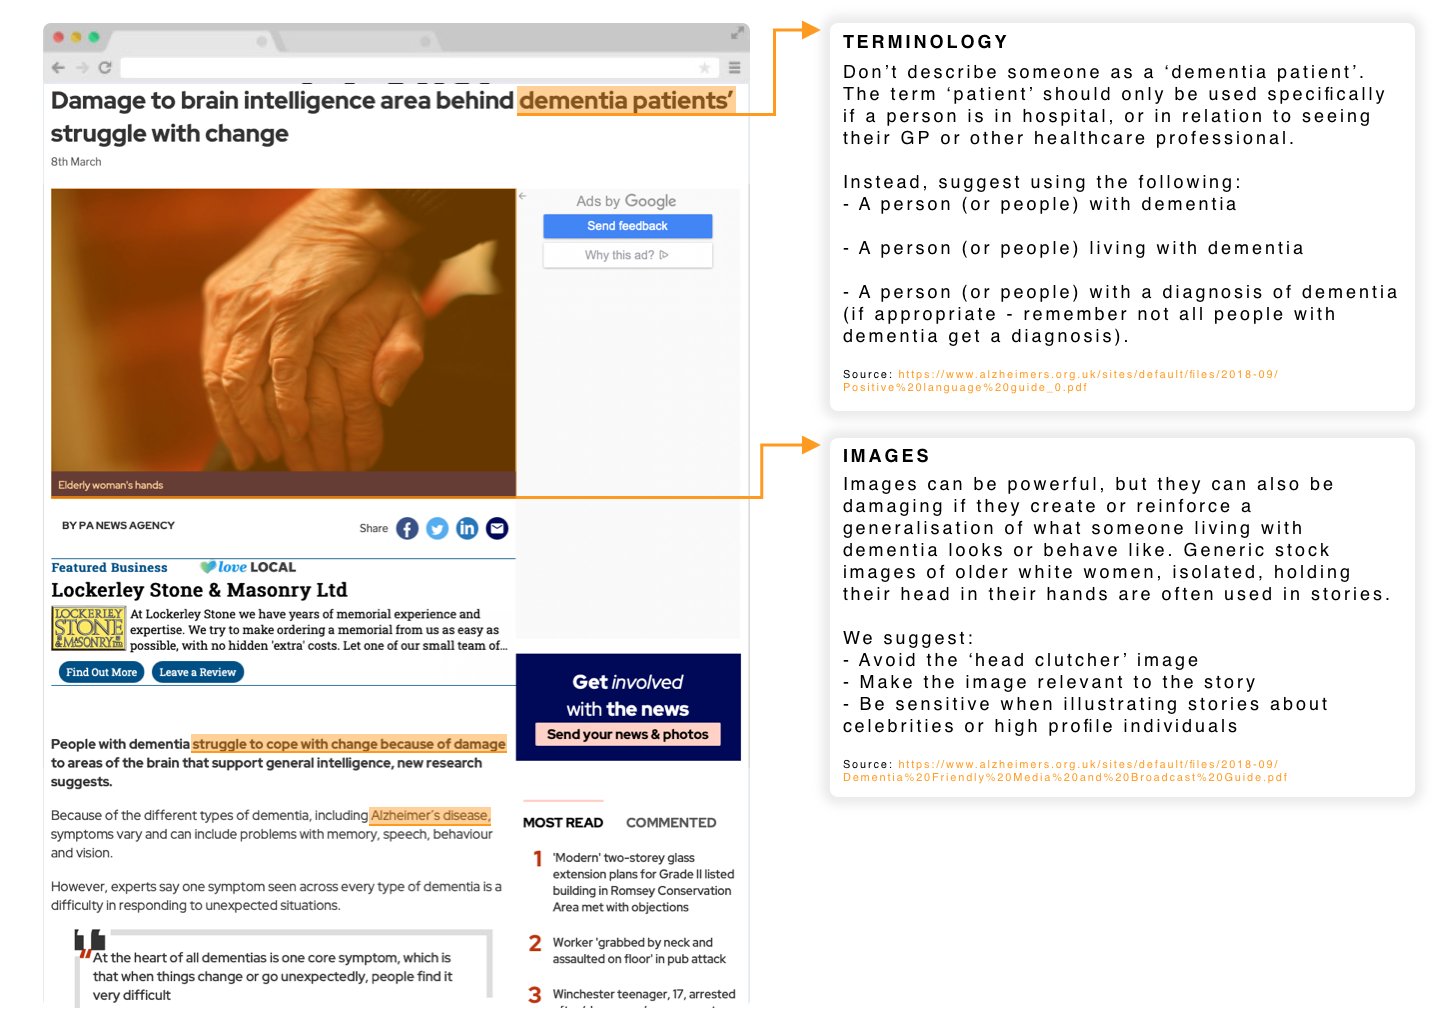
\includegraphics[width=1\linewidth]{Images/Discussion/Aware-AI.png}
\caption{Mockup of Suggestive guidance pack
 in action}
\label{fig:AwareAI}
\end{figure}
In the previous two chapters, I examined the ethical complexities that researchers, designers and developers face when designing with and for people with dementia. This work led to a series of unique insights into the ethical challenges of representing people with dementia and the co-creation of a lo-fi prototype toolkit for supporting communication and ethical decisions for designers, developers and people with dementia. One toolkit component that gained particular interest was 'suggestive guidance pack' found at reference. In this component, the tool would highlight negative labelling such as 'demented', or 'sufferer', and then suggest alternatives to improve the visual and textual representation of dementia (see how it may look like in fig.\ref{fig:AwareAI}). We could expand on this idea by \textit{\textbf{"exploring how AI may assist in the teaching and representing people with dementia"}}.

In recent years, AI-assisted tools have been widely used in the role of healthcare. These tools, have often been built to support the decision making of health records, insurance claims, and genome sequencing where the data is highly complex for human interpretation. \cite{lysaght2019ai} describes a series of ethical challenges that arise in AI-assisted decision-making. They emphasise the importance of \textit{"the public would have even greater confidence that decisions made in the complex ICU setting were carefully considered by experts and supported advanced technology"}. 

Lysaght raises important insights into AI decisions to have the necessary expertise back-up to provide confidence to whoever receives the information. Similarly, building upon the 'Suggestive Guidance Pack' found in chapter seven, people with dementia may be engaged with building the training data and guidance rules that the AI system build upon. For instance, people with dementia could vote and add recommendations for alternative suggestions for images that respectfully represent dementia.

In a similar vein to the early VR work found in chapter four, conducting work in AI and dementia may provide the opportunity to discover insights into how AI may support the social and political levels of dementia and HCI as opposed to the current stance of being used for pre-diagnostic and assessment studies. However, we must apply AI to social problems with an attentive and careful attitude, particularly when implementing the technology into sensitive settings that heavily rely on human contact and support. With this in mind, the future of AI design in dementia must require an interdisciplinary collaboration that is aware of the power relations amongst practitioners \citep{berridge2022design}.

\subsection{Nothing about us, without us}
\label{FutureStudyFour}
\begin{figure}[htp]
\centering
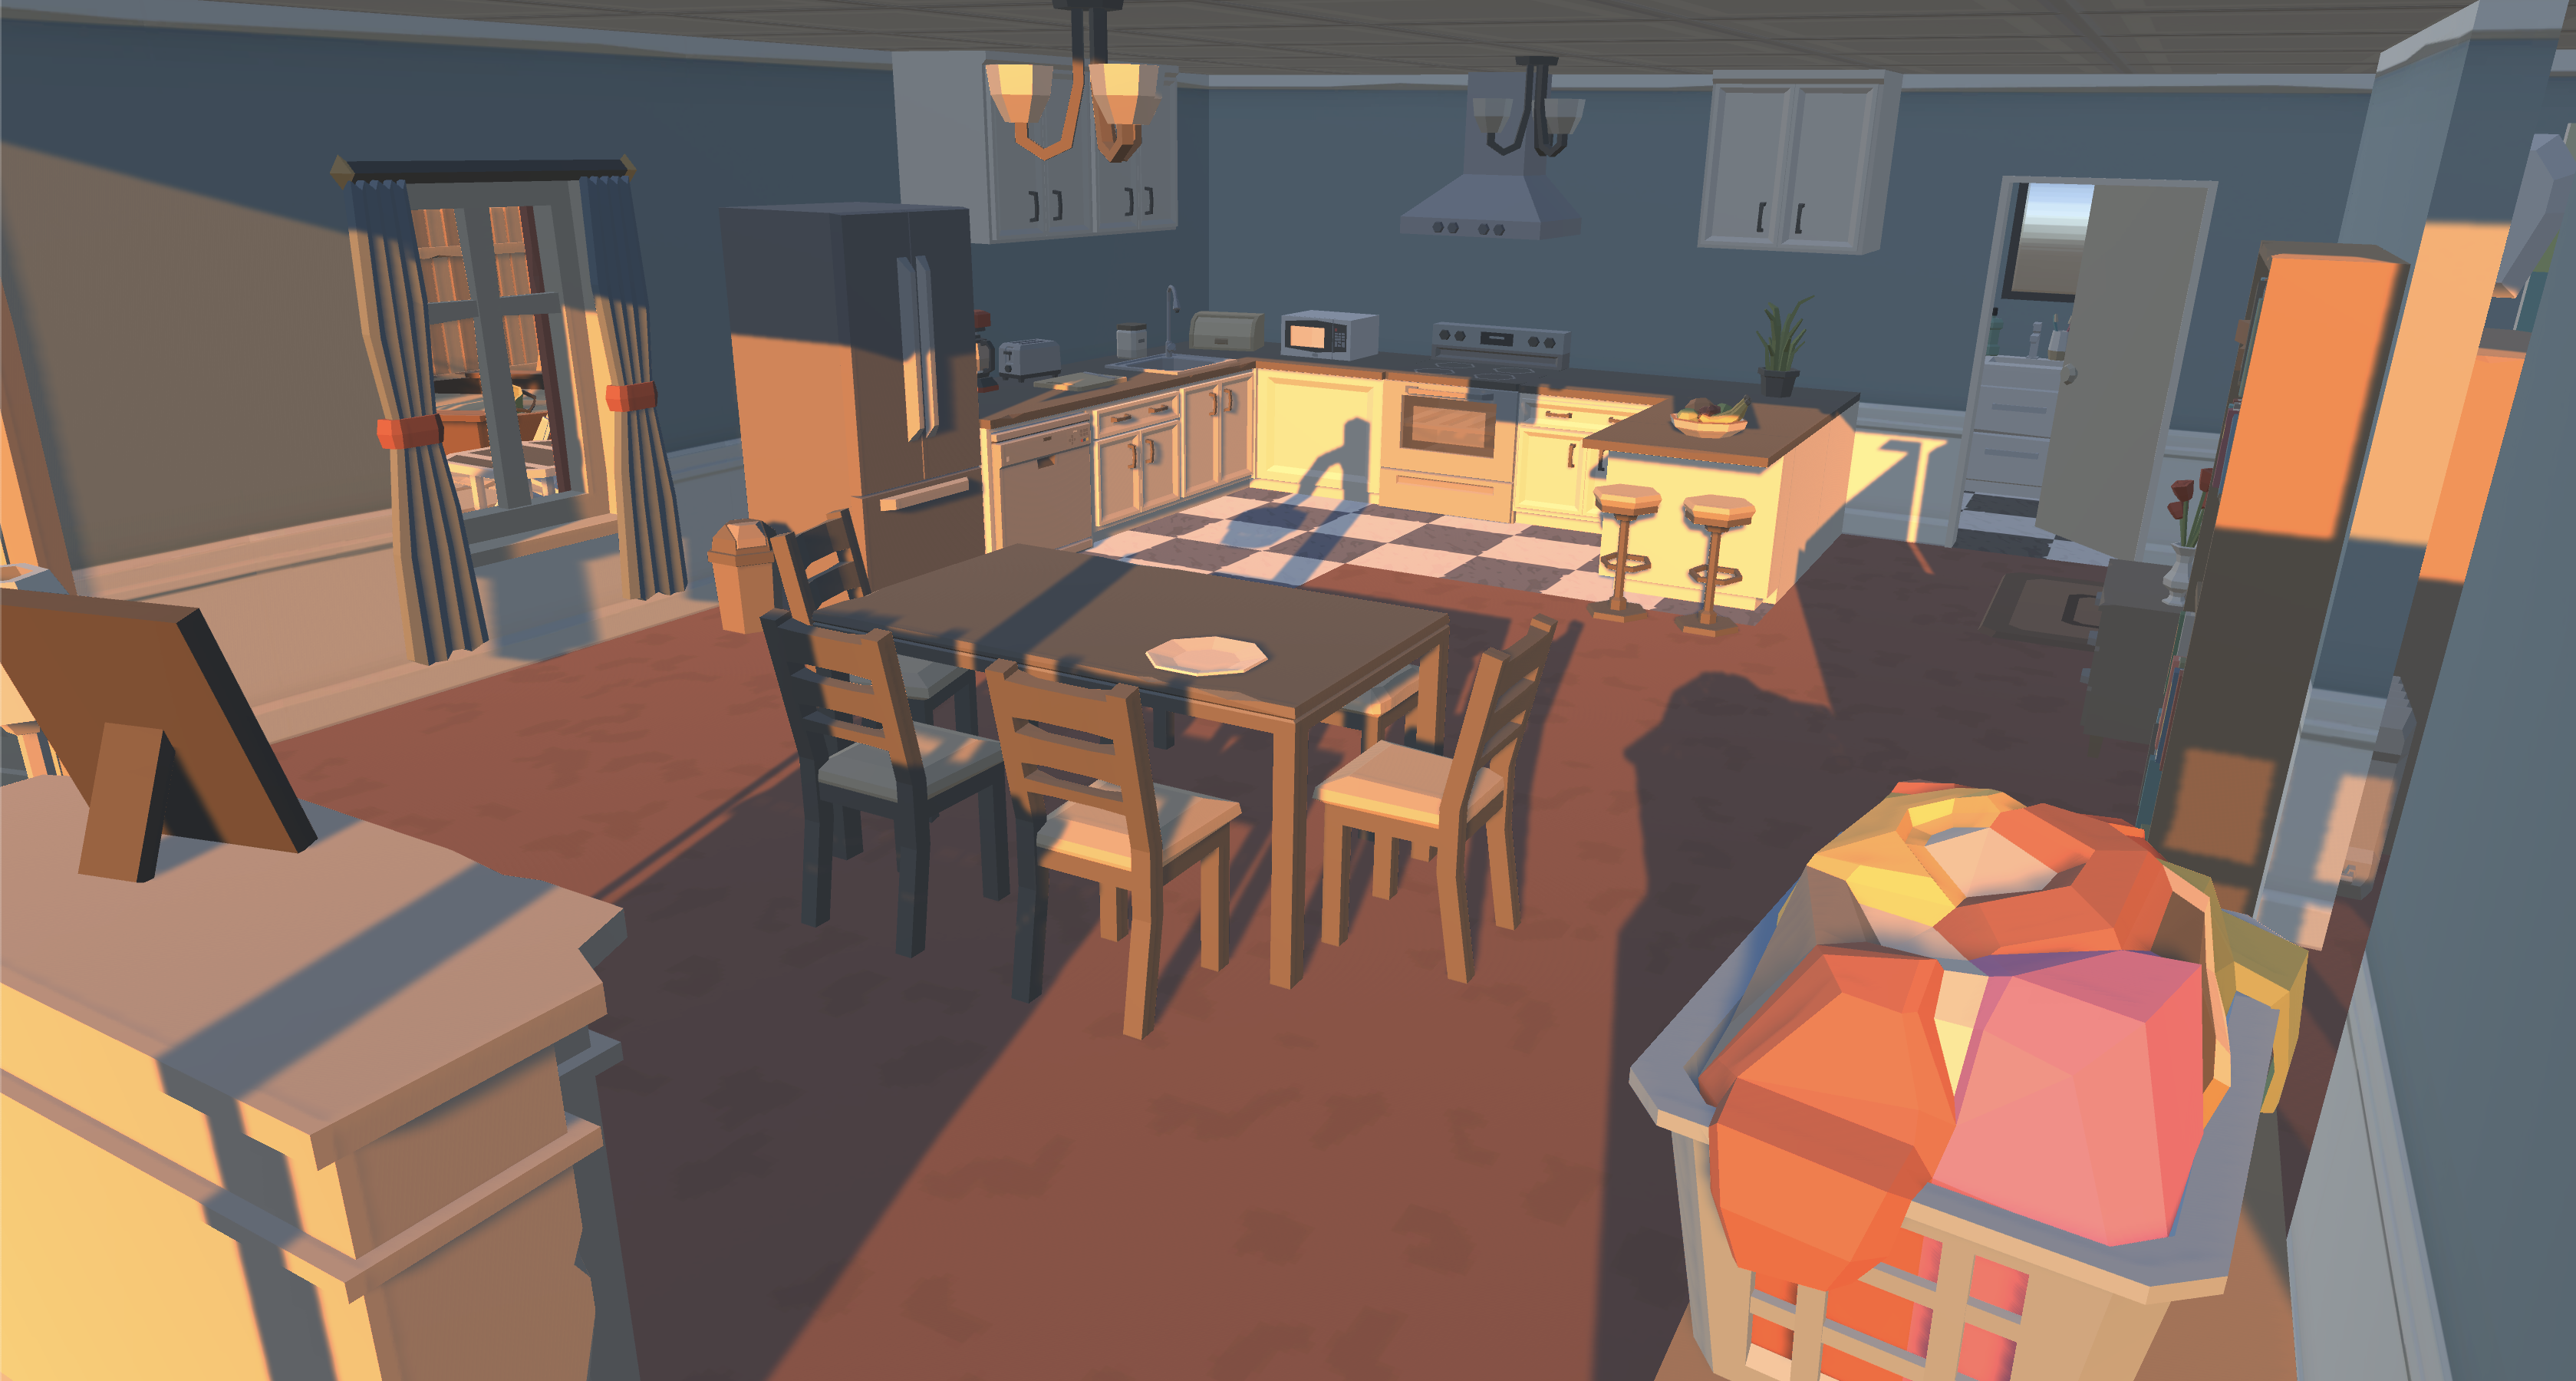
\includegraphics[width=1\linewidth]{Images/Discussion/Storytellling_Game.png}
\caption{Low-poly styling of a home for the game where the player can explore the person with dementia's story and learn about representation and stigma}
\label{fig:StorytellingLowPoly}
\end{figure}
In chapter seven's early stages of the toolkit, several workshops explored the idea of 'choose your own adventure' games to narrate the different experiences of dementia that will provide the public with immersive and meaningful explorations into what it means to live with dementia. Although this idea was not built upon in chapter seven, the use of games and other entertainment media formats may provide new ways to educate the public on the challenges and opportunities faced by experiences of dementia. 

Over the past decade, academia and best practice have presented a social and political perspective of what it means to live with dementia. However, while this may be a popular perspective, many academics or those within the dementia practice present within their work, this stance is radically different in the media portrayal. For instance, \cite{bailey2021battles} explored how media coverage influences the public attitudes of dementia, describing media draws on \textit{"biomedical discourse conceals alternative discourses and ideologies, such as a discourse of political and social action which would reinforce dementia as a global issue"}. The authors highlight this is often due to the emphasis on finding a cure which undermines the importance of care and the social environment for people with dementia. Likewise, movies and games have often followed the similar pursuit of prioritising the focus on the biomedical stance, whether that is using dementia as a 'disease' that the characters tackle throughout the movie, or a VR game to convey the challenges of living with dementia in hopes to provide funding for a cure.

In order to tackle representation issues in the media, researchers may want to \textit{\textbf{"explore how people with dementia may contribute to the design of media representation of dementia"}}. One concept researchers may want to look into is how we may design interactive games that have been co-created by people with dementia to construct the type of experiences and narrative that games may provide (mock-up image in figure \ref{fig:StorytellingLowPoly}). From chapter seven, it was apparent that people with dementia want to be and are necessary to expressing a genuine representing of dementia but requires many different insights into the uniqueness of living with dementia. As popularised by several dementia advocates and the disability movement, the phrase 'nothing about us, without us' \citep{spiel_nothing_2020} has become a popular saying and needs consideration in how media portrays dementia. This may be through a 'choose your own adventure game' to explore the different lives of people with dementia or act as a carer or friend to someone with dementia. While these types of media entertainment should focus on the discourse of living well with dementia to tackle the strong biomedical representation, I suggest we consider a more balanced view of the living with dementia that many of the participants I have worked with suggest. Additionally, although the living well with dementia perspective will develop a discourse that does not present a loss of agency, we must also acknowledge that they are challenges that come with dementia that requires necessary changes and alterations to the individuals', families', and friends' lives. 

\section{Final remarks}
\label{Discussion:FinalRemarks}
We have come a long way, and we have a long way to go. Within this thesis, the work has indicated tensions that arise in working within sensitive settings. As the work moved towards appreciating the importance of social relationships between people with dementia and others, it became apparent that new ways and practices are required to tell a fuller, relational story about experiences of dementia. For instance, in the early work of this PhD, I recognised the importance of the relationships between people with dementia are more than emotional support, but rather fruitful friendships to spend their days together. However, to extend the dialogue between the public and dementia (as I did in DemVR and toolkit), we require completely different structural factors to tackle stigma and discrimination while bridging the gap for discussions and voices to be heard. 

We all interact with the world differently. We communicate, experience, integrate ourselves differently from one another. Through relationships and learning from one another, we can move toward a more inclusive relationship and understanding of how our neighbours and communities can create meaning in their day-to-day experiences—regardless of their diagnosis. Although, as researchers in the field, we may understand that every person has personhood, this does not always seem apparent in the real world. Our next steps are to consider what it means to be an inclusive society, what it means to do inclusive research and to question the infrastructures that surround and often hold up our work.

 For instance, as researchers, how can we ensure ethical review boards are reflexive and dynamic when they are evaluating research that seeks to design in sensitive settings? This thesis stresses that we should take a more empathetic approach to our work which is echoed by others working in the field \citep{wallace_enabling_2012-1,lazar_safe_2019,morrissey_value_2017,kontos_integrating_2018}. To build upon the consensus of designing with people living with dementia, as researchers, we should aim to consider how we engage with the community from the very start of the research. In terms of those working in dementia, we should be engaging with advocates outside of HCI, such as organisations similar to Dementia Enquirers \citep{davies2021dementia}. Working with organisations similar to this can help to ensure that research agendas are more closely aligned with the needs of the population, thus moving toward a more inclusive approach to design and society. Ensuring our research designs are rooted in participant-led agendas can contribute to ethically engaged research impact. Finally, it is essential to note that deepening the narrative around dementia by introducing stories of friends, designers, developers, and the public will introduce a more fruitful perspective of everyday interactions for people with dementia. From here, we can start to consider ways for society to change and accommodate these new directions and representations of dementia instead of putting pressure on people with dementia to make the change.
